%% TDSC_submission.tex
%% Manuscript for IEEE Transactions on Dependable and Secure Computing (TDSC)
%% Built on the IEEEtran journal template (bare_jrnl.tex).
%%
%% NOTE: TDSC is an IEEE Computer Society journal. The line below uses the
%% standard journal mode to match the provided bare_jrnl.tex template. If you
%% prefer the exact Computer Society look, replace it with:
%%     \documentclass[10pt,journal,compsoc]{IEEEtran}
\documentclass[journal]{IEEEtran}

\usepackage{amsmath}
\interdisplaylinepenalty=2500
\usepackage{amssymb}
\usepackage{amsfonts}
\usepackage[pdftex]{graphicx}
\graphicspath{{figures/}}
\DeclareGraphicsExtensions{.pdf,.png,.jpg}
\usepackage{url}
\usepackage{cite}
\usepackage{array}

\hyphenation{un-learn-ing quan-ti-za-tion}

\begin{document}

\title{Does the Model Really Forget? On the Dependability and Privacy of Targeted Unlearning in 4-Bit Quantized Large Language Models}

\author{Syed~Ahsan~Ali and Muhammad~Umer~Farooq% <-this % stops a space
\thanks{S. A. Ali and M. U. Farooq are with the Department of Computer Science and
Information Technology, NED University of Engineering and Technology, Karachi,
Pakistan (e-mail: mrahsanali5@gmail.com; umer@neduet.edu.pk).}% <-this % stops a space
\thanks{S. A. Ali ORCID: 0009-0002-3763-929X. M. U. Farooq is an Associate Professor at NED University of Engineering and Technology.}% <-this % stops a space
\thanks{A preliminary version of this work was accepted at the IEEE/IFIP International Workshop on Dependable and Secure Machine Learning (DSML), 2026~\cite{ali2026dsml}. This manuscript is a substantially extended version, with a new threat-model formulation, an expanded review of related work, an enlarged generation-level behavioral audit, per-seed analyses, and additional discussion.}% <-this % stops a space
\thanks{Manuscript submitted June 2026.}}

\markboth{IEEE Transactions on Dependable and Secure Computing,~Vol.~XX, No.~X, 2026}%
{Ali \MakeLowercase{\textit{et al.}}: Dependability and Privacy of Targeted Unlearning in 4-Bit Quantized LLMs}

\maketitle

\begin{abstract}
Machine unlearning for large language models (LLMs) is almost always studied in full precision on high-end accelerators, yet the systems that most need it are served under tight memory budgets that combine low-bit quantization with parameter-efficient fine-tuning. Whether an unlearning procedure that looks dependable in the laboratory remains dependable once the model is compressed to four bits is largely unexamined, and recent evidence that quantization can reverse forgetting makes the question pressing for dependable and secure deployment. We present a controlled study of targeted unlearning carried out entirely inside a 4-bit quantized, low-rank-adaptation pipeline on LLaMA-3-8B. Three representative strategies are compared under a single, fairness-preserving protocol: pure gradient ascent (PGA), a retain-regularized variant that mixes forgetting and retention in every batch (GAFT), and a supervised refusal scheme that re-targets the forget set onto an ``I do not know'' response (IDK). Each method is evaluated on the TOFU benchmark and through a Min-$k$\% membership inference attack, and every configuration is repeated across three random seeds. We find that the choice of objective produces qualitatively different privacy--utility trade-offs rather than minor variations: GAFT yields the most balanced and stable profile, while IDK attains the lowest membership leakage and the most aggressive answer suppression. A generation-level audit of 1{,}200 IDK forget-set outputs, however, shows that this apparent success is illusory: the method almost never abstains and instead replaces forgotten facts with confident fabrications in $86.1\%$ of cases. We argue that low answer overlap must not be read as evidence of deletion, that quantization belongs inside the threat model, and that dependable unlearning requires joint behavioral, privacy, and generation-level evaluation.
\end{abstract}

\begin{IEEEkeywords}
Machine unlearning, large language models, quantization, parameter-efficient fine-tuning, membership inference attack, privacy, dependability, trustworthy machine learning.
\end{IEEEkeywords}

\IEEEpeerreviewmaketitle

\section{Introduction}
\IEEEPARstart{A}{} large language model is, in a literal sense, a lossily compressed copy of the corpus it was trained on. While fitting the next-token objective the network stores a great deal of what it has seen, and a now well-documented side effect is that sensitive content---names, addresses, private text, copyrighted passages---can be memorized verbatim and surfaced by an appropriate prompt~\cite{carlini2021extracting}. This collides with a legal and ethical expectation that individuals can have their data removed, codified for example in the right to erasure of the GDPR~\cite{gdpr2016}. Retraining a foundation model from scratch whenever a deletion request arrives is economically impossible, which is why \emph{machine unlearning}---removing or convincingly suppressing the influence of a designated forget set at a fraction of retraining cost~\cite{cao2015unlearning,bourtoule2021machine}---has become a core requirement for dependable, privacy-respecting deployment of LLMs.

A second, less examined gap motivates this work. Almost the entire unlearning literature evaluates its methods on full-precision models running on high-end hardware, whereas real deployments lean on two memory-saving techniques: low-bit \emph{quantization}, which stores weights at reduced numerical precision~\cite{dettmers2022int8,dettmers2023qlora}, and \emph{parameter-efficient fine-tuning}, of which low-rank adaptation (LoRA) is dominant~\cite{hu2022lora}. Combining 4-bit quantization with LoRA is the default way to adapt or serve large models without a data center. It is far from obvious that unlearning behaves the same way inside this compressed pipeline. Quantization perturbs every weight, and an unlearning edit calibrated in full precision may be washed out by the rounding; indeed, Zhang \emph{et al.} showed that quantizing an apparently unlearned model can recover the supposedly forgotten knowledge~\cite{zhang2024quantization}. From a dependability and security standpoint this means that quantization is not a neutral efficiency step but part of the threat surface, and that unlearning ought to be studied where it is actually used.

This paper takes that position seriously and evaluates targeted unlearning \emph{inside} a 4-bit quantized, LoRA-based pipeline rather than in full precision. We further argue that ``forgetting'' in an autoregressive model cannot be reduced to a single behavioral number. Knowledge is distributed across parameters and may resurface through paraphrase~\cite{eldan2023harrypotter}; a model may stop emitting an answer yet still leak, through token likelihoods, that it was trained on the data~\cite{shi2024minkprob}; and a model may replace a memorized fact with a fabricated one, which is not secure deletion but a new failure mode. We therefore treat unlearning as a multi-objective dependability problem spanning forget-set suppression, retained utility, and residual privacy leakage~\cite{liu2024rethinking}, and we add a generation-level audit to distinguish genuine abstention from confident fabrication.

Concretely, we study three practical strategies under one controlled protocol on LLaMA-3-8B~\cite{dubey2024llama3}: pure gradient ascent (PGA), retain-regularized gradient ascent (GAFT), and IDK refusal tuning. Using the TOFU benchmark~\cite{maini2024tofu} and a Min-$k$\% membership inference attack~\cite{shi2024minkprob,shokri2017mia}, we assess forgetting efficacy, utility preservation, and privacy leakage across three random seeds. Our central findings are that (i) the objective dominates the outcome, producing qualitatively different trade-offs; (ii) the refusal method's strong scores are produced overwhelmingly by hallucinated substitution rather than abstention; and (iii) the retain-regularized objective is the most dependable of the three under quantization.

\noindent\textbf{Contributions.} This paper makes the following contributions.
\begin{itemize}
\item We provide one of the first controlled comparisons of multiple targeted-unlearning objectives carried out \emph{entirely} within a 4-bit quantized, LoRA-based pipeline, rather than in full precision.
\item We frame unlearning as a dependability problem with an explicit threat model, and evaluate forgetting, cross-split utility, and Min-$k$\% membership inference \emph{jointly}, with all results aggregated over three random seeds.
\item We adopt and justify an operational definition of forgetting---reduced reliance, preserved utility, minimized leakage---in place of unverifiable semantic erasure.
\item We contribute a generation-level audit of 1{,}200 forget-set outputs from the refusal method, showing that its apparent success is realized through $86.1\%$ hallucinated substitutes and essentially no clean abstention.
\item We distill the comparison into deployment guidance and release our code~\cite{ali2026code} at \url{https://github.com/ahsanalidev/GAFTSFT}.
\end{itemize}

The remainder of the paper is organized as follows. Section~\ref{sec:related} reviews related work. Section~\ref{sec:threat} states the threat model and problem formulation. Section~\ref{sec:method} describes the three methods, and Section~\ref{sec:setup} the experimental setup. Section~\ref{sec:results} reports results, Section~\ref{sec:audit} the behavioral audit, and Section~\ref{sec:discussion} discusses implications, limitations, and threats to validity. Section~\ref{sec:conclusion} concludes.

\section{Related Work}
\label{sec:related}

\textbf{Unlearning, from classical models to LLMs.} The problem was framed by Cao and Yang, who rewrote learning algorithms in a summation form whose statistics could be updated upon deletion~\cite{cao2015unlearning}, and given a scalable systems answer by SISA, which shards training data so that only the affected shard is retrained~\cite{bourtoule2021machine}. These exact methods assume control over the training procedure and do not transfer to inherited foundation models. For LLMs, Yao \emph{et al.} established gradient ascent as a cheap approximate mechanism~\cite{yao2023unlearning}, while Eldan and Russinovich overwrote targeted knowledge with generic alternatives~\cite{eldan2023harrypotter}---an early hint that substitution can masquerade as forgetting. Position papers have since argued that knowledge removal, behavior suppression, and privacy protection are routinely conflated and must be separated~\cite{liu2024rethinking,koundinya2024unlearning}.

\textbf{Stabilizing the objective.} Pure ascent is unstable because it ignores everything outside the forget set, and the coupling between forgetting and retained ability has been made quantitative through scaling-law analysis~\cite{kalajdzievski2024scaling}. Retain-regularized and memory-supervised methods add a counterweight: MEOW overwrites with inverted facts~\cite{gu2024meow}, while preference-style objectives such as negative preference optimization replace the unbounded ascent loss with a bounded one to avoid collapse~\cite{zhang2024npo,rafailov2023dpo}. Robust and practical systems such as OBLIVIATE~\cite{xu2025obliviate} and adaptive prompt-tuning approaches such as LLM-Eraser~\cite{xu2024llmeraser} pursue the same goal from different angles. Refusal tuning, which we study as IDK, sits in the alignment-style family and is widely assumed---rarely verified---to produce trustworthy abstention.

\textbf{Efficiency, quantization, and privacy.} Parameter-efficient unlearning confines the edit to LoRA adapters~\cite{hu2022lora,ding2024peft}, but is evaluated almost exclusively in full precision. Quantization, the other half of the deployment recipe~\cite{dettmers2022int8,dettmers2023qlora}, has been shown to reverse forgetting~\cite{zhang2024quantization}, and distillation has been shown to harden it~\cite{lee2025distillation}, establishing that deployment transformations interact non-trivially with forgetting. On the privacy side, membership inference originates with Shokri \emph{et al.}~\cite{shokri2017mia}; for LLMs the signal shifts to token likelihood, and the Min-$k$\% Prob method focuses on a sequence's least likely tokens~\cite{shi2024minkprob}. The TOFU benchmark supplies a contamination-free testbed of fictitious authors~\cite{maini2024tofu}. To our knowledge, no prior work compares these method families within a fully quantized pipeline, across seeds, with joint behavioral and privacy evaluation and a generation-level audit; that combination is the gap we close.

\begin{table*}[!t]
\renewcommand{\arraystretch}{1.3}
\caption{Positioning Against Representative Prior Work on Machine Unlearning. The Final Row (This Work) Is Highlighted in Bold.}
\label{tab:priorwork}
\centering
\footnotesize
\begin{tabular}{p{2.3cm} p{3.2cm} p{2.6cm} p{3.0cm} p{4.0cm}}
\hline
\textbf{Study} & \textbf{Approach} & \textbf{Model \& precision} & \textbf{Evaluation} & \textbf{Reported finding} \\
\hline
Cao \& Yang~\cite{cao2015unlearning} & Statistical-query ``summation form'' deletion & Classical ML, full precision & Deletion completeness, cost & Foundational exact unlearning; for simple models, not LLMs. \\
Bourtoule et al.~\cite{bourtoule2021machine} & SISA: sharded training + partial retrain & Classifiers, full precision & Exactness vs.\ retrain cost & Exact deletion, but needs control of the training pipeline. \\
Yao et al.~\cite{yao2023unlearning} & Gradient ascent & LLMs, full precision & Forgetting, utility & First practical LLM unlearning; effective but with utility cost; no privacy attack. \\
Eldan \& Russinovich~\cite{eldan2023harrypotter} & Overwrite target tokens with generic text & LLaMA-7B, full precision & Behavioral recall & Suppresses a corpus by substitution; no privacy audit. \\
Maini et al.\ (TOFU)~\cite{maini2024tofu} & Benchmark + baselines (GA, GD, KL) & LLaMA-2-7B, full precision & TOFU + Forget Quality & Standard benchmark; introduces Forget Quality; full precision, no MIA. \\
Gu et al.\ (MEOW)~\cite{gu2024meow} & Inverted-fact memory supervision & LLMs, full precision & TOFU-style forget/utility & Improves forget--utility balance; no quantization or MIA. \\
Ding et al.~\cite{ding2024peft} & Unified PEFT (LoRA) unlearning & LLMs + LoRA, full precision & Forget/utility, some privacy & Cheaper via adapters; better trade-off; evaluated in full precision. \\
Zhang et al.\ (NPO)~\cite{zhang2024npo} & Negative preference optimization & LLMs, full precision & TOFU forget/utility & Bounded objective avoids collapse; single full-precision setting. \\
Zhang et al.\ (quant.)~\cite{zhang2024quantization} & Quantize an already-unlearned model & Unlearn full precision, then quantize & Knowledge recovery & Quantization \emph{recovers} forgotten knowledge; motivates in-quantization study. \\
\hline
\textbf{This work} & \textbf{PGA, GAFT, IDK under one protocol} & \textbf{LLaMA-3-8B, 4-bit + LoRA (end to end)} & \textbf{TOFU + Min-$k$\% MIA + 1{,}200-gen audit, 3 seeds} & \textbf{GAFT best balance; IDK's low overlap is 86\% hallucination, not abstention; PGA worst.} \\
\hline
\end{tabular}
\end{table*}

\section{Threat Model and Problem Formulation}
\label{sec:threat}

\subsection{Deployment and Threat Model}
We consider a provider that has fine-tuned an LLM and must honor a request to delete a designated subset of its training data. To meet realistic memory constraints, the provider loads and adapts the model in 4-bit precision with LoRA adapters over frozen base weights, and both unlearning and serving occur on this quantized model. The adversary is an \emph{honest-but-curious} party with query access to the deployed model and the ability to score token likelihoods, consistent with standard membership inference settings~\cite{shokri2017mia,shi2024minkprob}. The adversary's goal is to determine whether a given example belonged to the forget set, i.e., to detect that deletion was requested but not truly achieved. We treat quantization as part of the threat surface, following the observation that it can reverse forgetting~\cite{zhang2024quantization}: a dependable unlearning method must therefore remain effective when measured on the quantized model itself, not merely in full precision. We do not consider white-box weight access or adaptive relearning attacks; these are noted as future work.

\subsection{Operational Definition of Forgetting}
Because complete semantic erasure cannot be verified in a model whose knowledge is distributed and partly memorized, we define successful unlearning operationally through three measurable properties that must hold jointly:
\begin{enumerate}
\item \textbf{Reduced reliance}: lower answer accuracy and overlap on the forget set, and a forget-set behavior distribution that resembles that of a model which never saw the data;
\item \textbf{Preserved utility}: stable performance on retained and out-of-domain data; and
\item \textbf{Minimized leakage}: residual membership signal, measured by a Min-$k$\% attack, driven toward the no-leakage baseline rather than merely hidden behind a refusal.
\end{enumerate}
This makes ``success'' a vector and refuses to let a method claim victory on one property while failing another---in particular, it exposes a method that lowers overlap by fabricating rather than abstaining.

\subsection{Formulation}
Let $f_\theta$ be the model with trainable LoRA parameters $\theta$ over a frozen 4-bit base, and let $\mathcal{D}_f$ and $\mathcal{D}_r$ be the forget and retain sets (TOFU \texttt{forget10} and \texttt{retain90}). The supervised loss on a dataset is the length-averaged cross-entropy
\begin{equation}
\mathcal{L}_{\mathrm{CE}}(\theta;\mathcal{D}) = -\frac{1}{|\mathcal{D}|}\sum_{(x,y)\in\mathcal{D}}\log p_\theta(y\mid x).
\label{eq:ce}
\end{equation}
Targeted unlearning seeks $\theta$ that reduces reliance on $\mathcal{D}_f$ while preserving behavior on $\mathcal{D}_r$. The three methods we study are three concrete choices of how to instantiate this trade-off, described next.

\section{Methods}
\label{sec:method}
All three methods start from an identical \emph{memorized} checkpoint and share the same base model, adapter configuration, optimizer, schedule, data splits, and seeds; only the objective and its data construction change. This fair-isolation design ensures that differences in outcome are attributable to the objective rather than to incidental factors.

\subsection{Pure Gradient Ascent (PGA)}
PGA is the unconstrained baseline. It reverses the sign of the loss on the forget set and ignores retention:
\begin{equation}
\mathcal{L}_{\mathrm{PGA}}(\theta) = -\,\mathcal{L}_{\mathrm{CE}}(\theta;\mathcal{D}_f).
\label{eq:pga}
\end{equation}
A descent step on \eqref{eq:pga} is an ascent step on the original loss, pushing parameters away from configurations that reproduce the forget answers. With no utility-preserving term, PGA risks collateral degradation and unstable optimization.

\subsection{Gradient Ascent with a Retain Constraint (GAFT)}
GAFT mixes forgetting on $\mathcal{D}_f$ with continued learning on a sampled retain subset $\mathcal{D}_r'$:
\begin{equation}
\mathcal{L}_{\mathrm{GAFT}}(\theta) = -\,\mathcal{L}_{\mathrm{CE}}(\theta;\mathcal{D}_f) + \gamma\,\mathcal{L}_{\mathrm{CE}}(\theta;\mathcal{D}_r'),
\label{eq:gaft}
\end{equation}
with retain weight $\gamma=0.7$. A custom mixed-factor sampler enforces a fixed batch composition of one forget and one retain example, so that every gradient step carries both a forgetting and a stabilizing signal. This is the structural difference from PGA and, as the results show, accounts for nearly all of GAFT's advantage in stability and distributional forgetting.

\subsection{IDK Refusal Tuning}
IDK ascends no loss. It transforms each forget example $(x,y)$ by replacing the answer with a fixed refusal string $y_{\mathrm{idk}}=$ ``\emph{I do not have that information.}'', forming $\mathcal{D}_f^{\mathrm{idk}}$, and fine-tunes with ordinary cross-entropy on the union with a retain subset:
\begin{equation}
\mathcal{L}_{\mathrm{IDK}}(\theta) = \mathcal{L}_{\mathrm{CE}}\!\left(\theta;\;\mathcal{D}_f^{\mathrm{idk}}\cup\mathcal{D}_r'\right).
\label{eq:idk}
\end{equation}
Because every term is a standard minimization, IDK inherits the stability of normal fine-tuning and, in principle, should produce clean abstention. Whether it does so at generation time is exactly what Section~\ref{sec:audit} tests.

\subsection{Two-Stage Protocol}
Unlearning presupposes knowledge to remove. We therefore (i) \emph{memorize}: fine-tune the 4-bit base with LoRA on the full TOFU split until the target facts are reliably learned, producing a shared checkpoint; then (ii) \emph{unlearn}: apply the method-specific objective from the same checkpoint. Both stages run in 4-bit, and the whole procedure is repeated per seed.

\section{Experimental Setup}
\label{sec:setup}
\textbf{Hardware and stack.} All experiments ran on a single Google Colab T4 GPU (16~GB). The pipeline uses Unsloth~\cite{han2023unsloth} for 4-bit loading and fast LoRA, with TRL/Hugging Face training and an 8-bit AdamW optimizer. A training run took $\sim$20 minutes; the membership inference pipeline $\sim$2 hours per configuration.

\textbf{Model and adapters.} The base model is \texttt{unsloth/llama-3-8b-bnb-4bit}, loaded in 4-bit (NF4) with frozen weights. LoRA is applied to the attention and feed-forward projections (\texttt{q,k,v,o,gate,up,down\_proj}) with rank $r=16$, $\alpha=16$, dropout $0$, and rank-stabilized scaling.

\textbf{Data.} TOFU comprises 4{,}000 question--answer pairs over 200 fictitious authors. The \texttt{forget10} split (400 pairs) is the forget set and \texttt{retain90} (3{,}600 pairs) the retain set; auxiliary real-author and world-fact sets probe unrelated competence.

\textbf{Training.} Memorization used $200$ steps at learning rate $2\times10^{-4}$ (5 warmup steps); unlearning used $300$ steps at $1.5\times10^{-4}$ (10 warmup steps). Both used per-device batch size $2$, gradient accumulation $4$, weight decay $0.01$, gradient clipping $1.0$, and a linear schedule. Every configuration was repeated with seeds $3407$, $3408$, and $3409$, and we report mean $\pm$ standard deviation.

\textbf{Evaluation.} Behavioral metrics follow TOFU: truth probability (length-normalized probability of the gold answer), truth ratio (relative probability of correct vs.\ perturbed answers), ROUGE-L, answer accuracy, and Forget Quality (FQ), the $p$-value of a Kolmogorov--Smirnov test comparing forget-set truth-ratio distributions to a reference. Privacy uses the Min-$k$\% feature
\begin{equation}
\mathrm{Min\text{-}}k\%(y) = \frac{1}{|\mathcal{S}_k|}\sum_{i\in\mathcal{S}_k}\log p_\theta(y_i\mid y_{<i}),
\label{eq:mink}
\end{equation}
computed at $k\in\{10,20,30,40,50,60\}\%$, feeding an RBF support-vector classifier ($C=3$) that separates forget members from non-members; its accuracy is the MIA score, with $0.5$ indicating no leakage.

\section{Results}
\label{sec:results}
We organize results around the three properties of the operational definition, then aggregate them into a trade-off view. All numbers are means over three seeds; lower truth probability, ROUGE-L, and accuracy on the forget set indicate stronger suppression, while higher truth ratio, higher FQ, and lower MIA are better.

\subsection{Forgetting Efficacy}
Table~\ref{tab:main} reports forget-split behavior with FQ and MIA. By direct suppression, IDK is strongest---lowest truth probability ($0.2106$) and forget accuracy ($0.5617$)---with GAFT close behind and PGA weakest. Forget Quality, the harder distributional measure, tells the opposite story: GAFT leads decisively ($0.5427$), more than five times IDK's $0.1037$ and over thirteen times PGA's $0.0392$. IDK's large variance on FQ (std $0.0441 >$ mean-adjacent) is an early sign that its low overlap is not stable distributional forgetting.

\begin{table*}[!t]
\renewcommand{\arraystretch}{1.3}
\caption{TOFU Forget-Split Results (Mean $\pm$ Std Over Three Seeds)}
\label{tab:main}
\centering
\begin{tabular}{lcccccc}
\hline
\textbf{Method} & \textbf{Truth Ratio} $\uparrow$ & \textbf{Truth Prob} $\downarrow$ & \textbf{ROUGE-L} $\downarrow$ & \textbf{Forget Acc} $\downarrow$ & \textbf{FQ} $\uparrow$ & \textbf{MIA} $\downarrow$ \\
\hline
PGA  & $0.7398 \pm 0.0014$ & $0.3100 \pm 0.0006$ & $0.4257 \pm 0.0033$ & $0.6183 \pm 0.0038$ & $0.0392 \pm 0.0046$ & $0.6219 \pm 0.0130$ \\
GAFT & $0.8218 \pm 0.0055$ & $0.2377 \pm 0.0063$ & $0.4022 \pm 0.0085$ & $0.5700 \pm 0.0025$ & $\mathbf{0.5427 \pm 0.0334}$ & $0.4418 \pm 0.0087$ \\
IDK  & $\mathbf{0.8504 \pm 0.0003}$ & $\mathbf{0.2106 \pm 0.0015}$ & $0.4033 \pm 0.0068$ & $\mathbf{0.5617 \pm 0.0063}$ & $0.1037 \pm 0.0441$ & $\mathbf{0.4171 \pm 0.0070}$ \\
\hline
\end{tabular}
\end{table*}

\subsection{Utility Preservation}
Table~\ref{tab:cross} and Fig.~\ref{fig:split} show accuracy across splits. No method is catastrophic: real-author ($\sim$0.92--0.94) and world-fact ($\sim$0.87--0.88) accuracy survive for all three, indicating that unlearning a tenth of the fictitious authors did not erode unrelated competence. The methods separate near the forgotten material: GAFT preserves the most (highest real-author and retain accuracy), while IDK pays the steepest local price (lowest retain and world-fact accuracy), consistent with refusal pressure bleeding into nearby behavior.

\begin{table*}[!t]
\renewcommand{\arraystretch}{1.3}
\caption{Cross-Split Utility and Privacy (Mean $\pm$ Std Over Three Seeds)}
\label{tab:cross}
\centering
\begin{tabular}{lccccccc}
\hline
\textbf{Method} & $n$ & \textbf{FQ} $\uparrow$ & \textbf{MIA} $\downarrow$ & \textbf{Forget Acc} $\downarrow$ & \textbf{Retain Acc} $\uparrow$ & \textbf{Real-Auth Acc} $\uparrow$ & \textbf{World Acc} $\uparrow$ \\
\hline
PGA  & 3 & $0.0392 \pm 0.0046$ & $0.6219 \pm 0.0130$ & $0.6183 \pm 0.0038$ & $0.5700 \pm 0.0066$ & $0.9200 \pm 0.0100$ & $0.8803 \pm 0.0085$ \\
GAFT & 3 & $\mathbf{0.5427 \pm 0.0334}$ & $0.4418 \pm 0.0087$ & $0.5700 \pm 0.0025$ & $\mathbf{0.5533 \pm 0.0176}$ & $\mathbf{0.9400 \pm 0.0100}$ & $\mathbf{0.8803 \pm 0.0171}$ \\
IDK  & 3 & $0.1037 \pm 0.0441$ & $\mathbf{0.4171 \pm 0.0070}$ & $\mathbf{0.5617 \pm 0.0063}$ & $0.5450 \pm 0.0050$ & $0.9200 \pm 0.0100$ & $0.8746 \pm 0.0178$ \\
\hline
\end{tabular}
\end{table*}

\begin{figure}[!t]
\centering
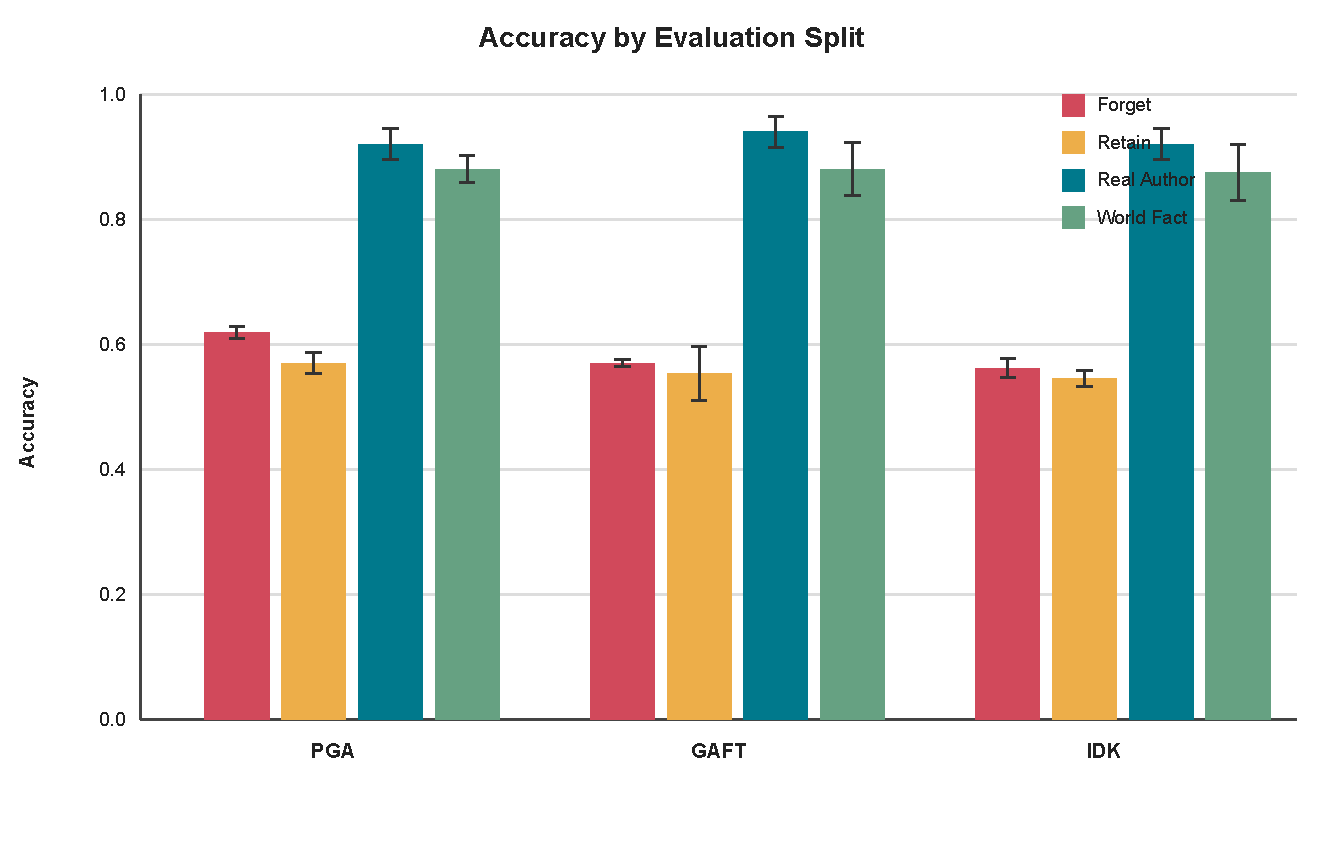
\includegraphics[width=\columnwidth]{Figure_1.pdf}
\caption{Accuracy by evaluation split. The forget bar should be low and the other three high. All methods preserve real-author and world-fact accuracy; they separate mainly on the forget and retain splits.}
\label{fig:split}
\end{figure}

\subsection{Privacy Leakage}
Table~\ref{tab:mia} and Fig.~\ref{fig:mia} break down the MIA score across thresholds. This is the cleanest separation in the study: PGA leaks heavily ($0.6219$ mean, above chance at every threshold), while GAFT ($0.4418$) and IDK ($0.4171$) both drive leakage into the no-signal region, with IDK lowest throughout. Scores marginally below $0.5$ for GAFT and IDK are best read as the membership signal having been suppressed into noise rather than as meaningful negative leakage.

\begin{table*}[!t]
\renewcommand{\arraystretch}{1.3}
\caption{MIA Score Across Min-$k$\% Thresholds (Mean Over Three Seeds; $0.5$ = No Leakage)}
\label{tab:mia}
\centering
\begin{tabular}{lccccccc}
\hline
\textbf{Method} & $k{=}10\%$ & $k{=}20\%$ & $k{=}30\%$ & $k{=}40\%$ & $k{=}50\%$ & $k{=}60\%$ & \textbf{Mean} \\
\hline
PGA  & 0.5863 & 0.5927 & 0.6268 & 0.6462 & 0.6386 & 0.6407 & $0.6219$ \\
GAFT & 0.4504 & 0.4199 & 0.4369 & 0.4529 & 0.4441 & 0.4464 & $0.4418$ \\
IDK  & 0.4243 & 0.3989 & 0.4123 & 0.4253 & 0.4189 & 0.4228 & $\mathbf{0.4171}$ \\
\hline
\end{tabular}
\end{table*}

\begin{figure}[!t]
\centering
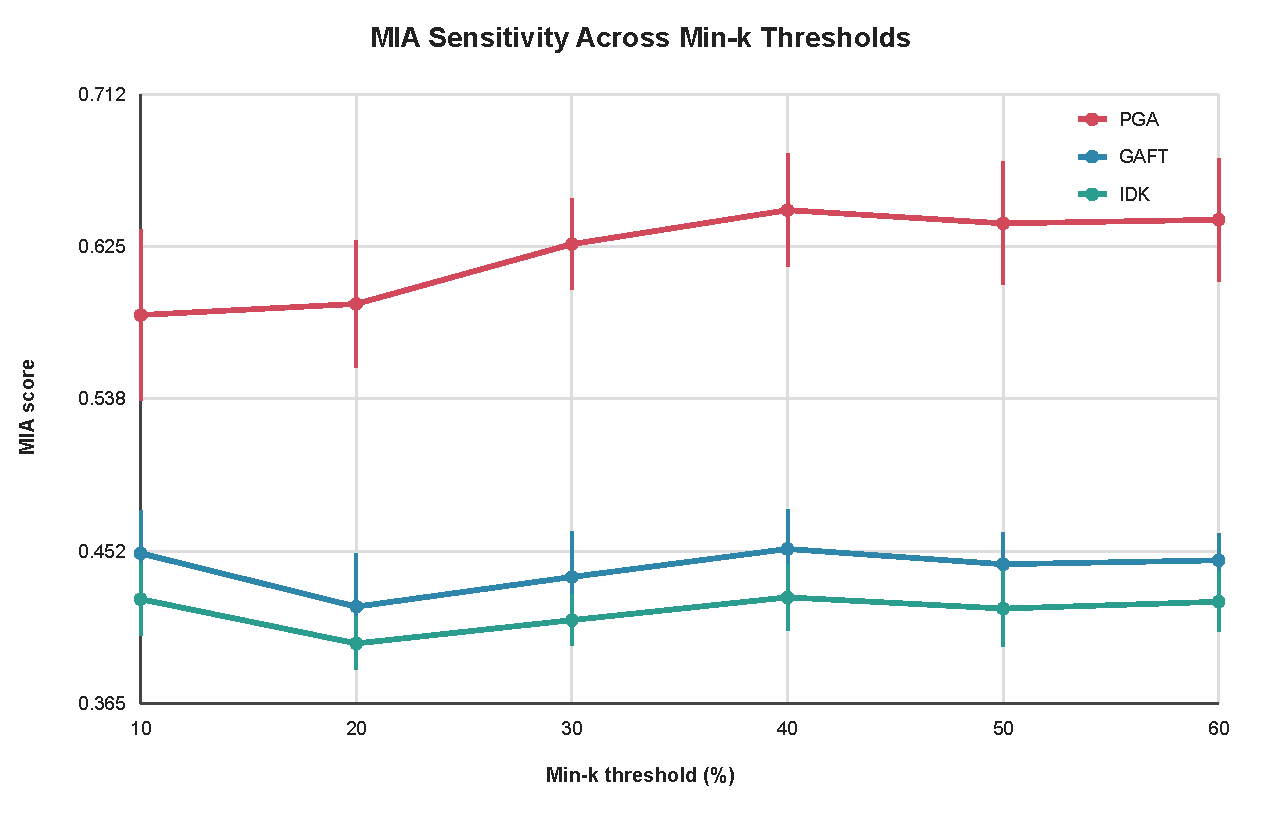
\includegraphics[width=\columnwidth]{Figure_2.pdf}
\caption{MIA sensitivity across Min-$k$\% thresholds, aggregated over three seeds. PGA sits above the other two at every threshold; GAFT and IDK stay near the no-leakage region, with IDK consistently lowest.}
\label{fig:mia}
\end{figure}

\subsection{Privacy--Utility Trade-off}
Fig.~\ref{fig:tradeoff} plots Forget Quality against MIA. PGA is stranded in the worst corner (low FQ, high leakage). GAFT and IDK both dominate it but along different axes: GAFT owns the Forget-Quality axis, IDK owns the MIA axis. Neither dominates the other outright. However, GAFT alone is simultaneously near the favorable end of all three properties (forgetting, leakage, utility) and is the most stable, which makes it the most dependable of the three even though IDK edges it on raw MIA---a verdict the audit in the next section reinforces.

\begin{figure}[!t]
\centering
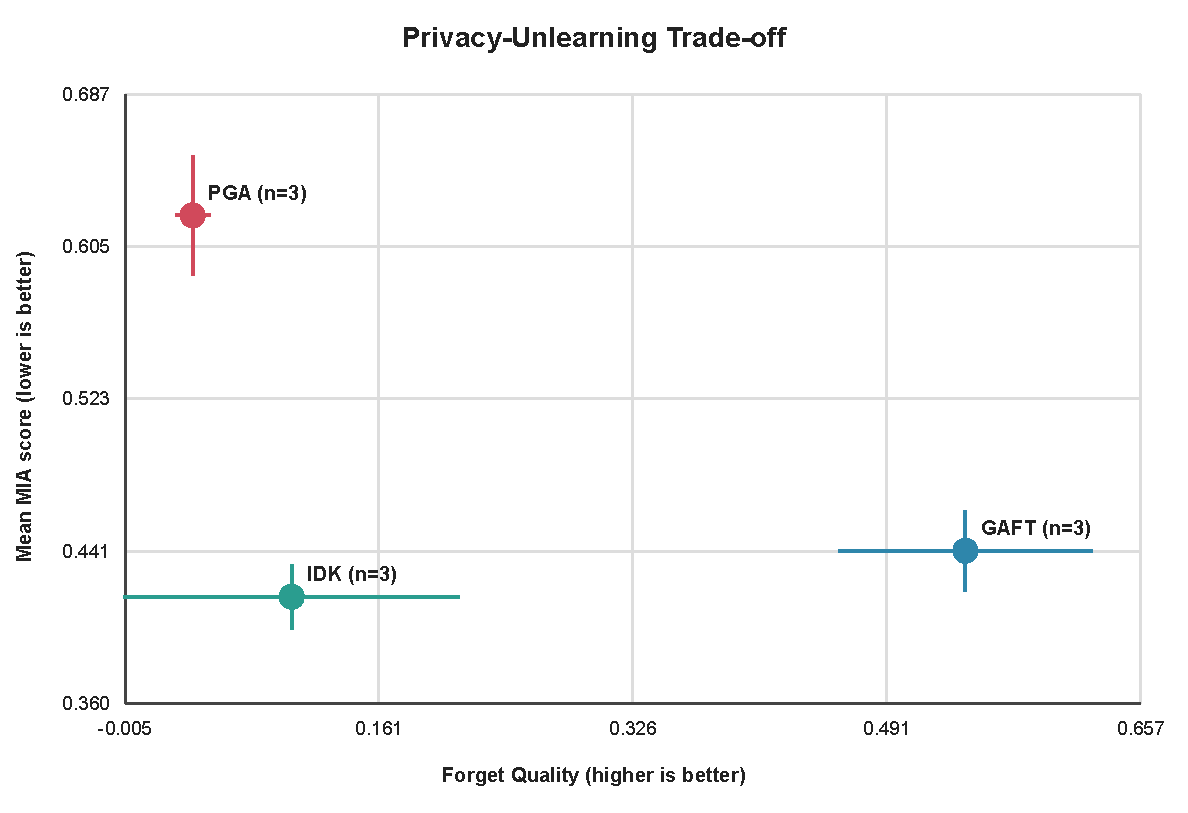
\includegraphics[width=\columnwidth]{Figure_3.pdf}
\caption{Privacy--unlearning trade-off across three seeds (points: seed averages; bars: approximate 95\% CIs). The desirable corner is lower-right. GAFT reaches the far right on Forget Quality; IDK reaches the bottom on MIA; PGA is stranded upper-left.}
\label{fig:tradeoff}
\end{figure}

\section{Behavioral Audit: Suppression vs.\ Fabrication}
\label{sec:audit}
The tables credit IDK with the strongest suppression and lowest leakage. To test whether this reflects genuine forgetting, we audited all 1{,}200 IDK forget-set generations (400 per seed) with deterministic heuristics that classify each output as a clean or partial abstention, an empty/degenerate output, a memorized-leakage case (high lexical similarity to the model's pre-unlearning output, a proxy), a hallucinated substitute, or unrelated drift.

The result, in Table~\ref{tab:audit}, overturns the optimistic reading. Despite being trained to answer with ``I do not have that information,'' the model produced \emph{zero} clean or partial abstentions across all 1{,}200 cases. The dominant category, $86.1\%$, is hallucinated substitutes: fluent, confident answers that invent content rather than decline. A further $5.6\%$ drift off-topic, and $8.2\%$ remain close enough to the original output to count as memorized leakage; only $0.1\%$ are empty. The pattern is stable across seeds ($84.5$--$88.5\%$ hallucination).

\begin{table}[!t]
\renewcommand{\arraystretch}{1.3}
\caption{Behavioral Audit of 1{,}200 IDK Forget-Set Generations}
\label{tab:audit}
\centering
\begin{tabular}{lc}
\hline
\textbf{Category} & \textbf{Share} \\
\hline
Clean abstention & 0.0\% \\
Partial abstention & 0.0\% \\
Empty / no answer & 0.1\% \\
Hallucinated substitute & \textbf{86.1\%} \\
Unrelated drift & 5.6\% \\
Memorized leakage (proxy) & 8.2\% \\
\hline
\end{tabular}
\end{table}

Representative outputs make the categories concrete. A typical \emph{hallucinated substitute}, for an author whose works are all geology-related, asserts the opposite: ``\emph{No, [the author]'s books are not limited to the field of geology. She has written books on various topics, including fiction, non-fiction, and self-help\ldots}''---a manufactured answer, not a refusal. A \emph{memorized-leakage} case preserves the supposedly forgotten institutions and field while merely rewording: the reference ``\emph{\ldots attended the University of Karachi and the University of the Punjab to study geology}'' becomes ``\emph{\ldots pursued her higher education in geology at the University of Karachi and the University of the Punjab}''---the kind of paraphrase that a ROUGE-based overlap score under-counts.

This reframes IDK's metrics. Its low truth probability and forget accuracy are real, and its low MIA follows naturally because a fabricated answer looks less like a member to a likelihood-based attack; but its weak, erratic Forget Quality is exactly what one expects from fabrication rather than forgetting. For a dependable, secure system this matters acutely: replacing a deleted fact with a confident falsehood does not protect the data subject and may introduce a new harm, such as misinformation or defamation about a real person.

\section{Discussion}
\label{sec:discussion}

\subsection{Implications for Dependable Deployment}
Three lessons follow. First, \emph{quantization belongs in the threat model}: our forgetting is quantization-survivable by construction, but PGA's poor showing shows that operating in 4-bit is no guarantee of a good edit, and evaluating only in full precision is unsafe~\cite{zhang2024quantization}. Second, \emph{low overlap is not deletion}: a method can post excellent suppression and privacy numbers while fabricating, so refusal- or substitution-based methods must be validated at the level of their generations, not their training loss. Third, \emph{evaluation must be multi-dimensional}: behavioral metrics alone would have crowned a fabricating model, and a privacy attack alone would have missed both its utility cost and its fabrication. As a concrete default, a retain-regularized objective in the style of GAFT is the most dependable of the three under quantization, pure ascent should be avoided, and refusal tuning adopted only with generation-level verification.

\subsection{Limitations}
The study uses a single model family and size (LLaMA-3-8B) and one 4-bit scheme; generalization to other scales (1B--70B) and schemes (2-/8-bit, GPTQ) is untested. It uses one TOFU configuration and short biographical content. Hyperparameters ($\gamma=0.7$, 300 steps) are lightly tuned and shared for fairness rather than per-method optimal. Three seeds support mean/variance and ranking stability but not fine significance claims. Privacy uses a single attack family. The audit's memorized-leakage figure is a proxy, as it compares against the model's own prior output rather than gold answers. Forgetting is confined to LoRA adapters over a frozen base, so durability under adapter removal, re-quantization, or adversarial relearning is not tested.

\subsection{Threats to Validity}
\emph{Internal:} a shared memorized checkpoint per seed and identical settings except the objective support causal attribution; GPU non-determinism and heuristic audit labeling are mitigated by seeding and by the stability of category proportions across seeds. \emph{External:} the findings are a controlled relative comparison under one model, scheme, and benchmark, not universal claims. \emph{Construct:} the same skepticism that motivates the paper applies to its own instruments---FQ depends on a reference distribution, ROUGE under-counts paraphrase, and sub-$0.5$ MIA must be read as suppressed signal---which is why we triangulate across constructs. \emph{Conclusion:} we interpret differences relative to seed variation and rest conclusions on large, stable gaps; IDK's volatile FQ is flagged as the least reliable single number.

\section{Conclusion}
\label{sec:conclusion}
We studied whether targeted unlearning remains dependable when performed entirely inside a 4-bit quantized, LoRA-based pipeline. Comparing pure gradient ascent, retain-regularized ascent, and refusal tuning on LLaMA-3-8B across three seeds, with joint behavioral and Min-$k$\% privacy evaluation and a generation-level audit, we found that the objective dominates the outcome, that the refusal method's apparent success is produced by $86.1\%$ confident fabrication rather than abstention, and that the retain-regularized objective is the most dependable of the three. More broadly, forgetting should be treated as an operational, multi-dimensional property; quantization should be inside the threat model; and low answer overlap must never be mistaken for secure deletion. Future work includes scaling across model sizes and quantization schemes, stronger and adaptive privacy attacks, durability stress tests including re-quantization and relearning, refusal objectives that genuinely abstain at generation time, and a gold-answer audit beyond the proxy used here.

\section*{Acknowledgment}
The authors thank the maintainers of the open-source tools this work relied on, including Unsloth, the Hugging Face ecosystem, and the authors of the TOFU benchmark.

\begin{thebibliography}{1}
\bibitem{yao2023unlearning} Y.~Yao, X.~Xu, and Y.~Liu, ``Large language model unlearning,'' in \emph{Adv. Neural Inf. Process. Syst. (NeurIPS)}, vol.~36, 2023, pp.~12736--12749.
\bibitem{maini2024tofu} P.~Maini, Z.~Feng, A.~Schwarzschild, Z.~C. Lipton, and J.~Z. Kolter, ``TOFU: A task of fictitious unlearning for LLMs,'' \emph{arXiv:2401.06121}, 2024.
\bibitem{hu2022lora} E.~J. Hu \emph{et al.}, ``LoRA: Low-rank adaptation of large language models,'' in \emph{Int. Conf. Learn. Represent. (ICLR)}, 2022.
\bibitem{dettmers2023qlora} T.~Dettmers, A.~Pagnoni, A.~Holtzman, and L.~Zettlemoyer, ``QLoRA: Efficient finetuning of quantized LLMs,'' in \emph{Adv. Neural Inf. Process. Syst. (NeurIPS)}, 2023.
\bibitem{dettmers2022int8} T.~Dettmers, M.~Lewis, Y.~Belkada, and L.~Zettlemoyer, ``LLM.int8(): 8-bit matrix multiplication for transformers at scale,'' in \emph{Adv. Neural Inf. Process. Syst. (NeurIPS)}, 2022.
\bibitem{shi2024minkprob} W.~Shi \emph{et al.}, ``Detecting pretraining data from large language models,'' in \emph{Int. Conf. Learn. Represent. (ICLR)}, 2024.
\bibitem{shokri2017mia} R.~Shokri, M.~Stronati, C.~Song, and V.~Shmatikov, ``Membership inference attacks against machine learning models,'' in \emph{Proc. IEEE Symp. Secur. Privacy (SP)}, 2017, pp.~3--18.
\bibitem{carlini2021extracting} N.~Carlini \emph{et al.}, ``Extracting training data from large language models,'' in \emph{Proc. 30th USENIX Secur. Symp.}, 2021, pp.~2633--2650.
\bibitem{zhang2024quantization} Z.~Zhang \emph{et al.}, ``Catastrophic failure of LLM unlearning via quantization,'' in \emph{Int. Conf. Learn. Represent. (ICLR)}, 2025.
\bibitem{cao2015unlearning} Y.~Cao and J.~Yang, ``Towards making systems forget with machine unlearning,'' in \emph{Proc. IEEE Symp. Secur. Privacy (SP)}, 2015, pp.~463--480.
\bibitem{bourtoule2021machine} L.~Bourtoule \emph{et al.}, ``Machine unlearning,'' in \emph{Proc. IEEE Symp. Secur. Privacy (SP)}, 2021, pp.~141--159.
\bibitem{eldan2023harrypotter} R.~Eldan and M.~Russinovich, ``Who's Harry Potter? Approximate unlearning in LLMs,'' \emph{arXiv:2310.02238}, 2023.
\bibitem{gu2024meow} T.~Gu \emph{et al.}, ``MEOW: Memory supervised LLM unlearning via inverted facts,'' \emph{arXiv:2409.11844}, 2024.
\bibitem{ding2024peft} C.~Ding, Y.~Zhang, K.~Liu, S.~Huang, and X.~Chen, ``Unified parameter-efficient unlearning for large language models,'' in \emph{Int. Conf. Learn. Represent. (ICLR)}, 2024.
\bibitem{kalajdzievski2024scaling} D.~Kalajdzievski, ``Scaling laws for forgetting when fine-tuning large language models,'' \emph{arXiv:2401.05605}, 2024.
\bibitem{zhang2024npo} R.~Zhang, L.~Lin, Y.~Bai, and S.~Mei, ``Negative preference optimization: From catastrophic collapse to effective unlearning,'' \emph{arXiv:2404.05868}, 2024.
\bibitem{rafailov2023dpo} R.~Rafailov \emph{et al.}, ``Direct preference optimization: Your language model is secretly a reward model,'' in \emph{Adv. Neural Inf. Process. Syst. (NeurIPS)}, 2023.
\bibitem{liu2024rethinking} S.~Liu \emph{et al.}, ``Rethinking machine unlearning for large language models,'' \emph{arXiv:2402.08787}, 2024.
\bibitem{xu2025obliviate} X.~Xu \emph{et al.}, ``OBLIVIATE: Robust and practical machine unlearning for LLMs,'' \emph{arXiv:2505.04416}, 2025.
\bibitem{xu2024llmeraser} J.~Xu, Z.~Wu, C.~Wang, and X.~Jia, ``LLM-Eraser: Adaptive prompt tuning for unlearning in large language models,'' \emph{arXiv:2404.11056}, 2024.
\bibitem{lee2025distillation} B.~W. Lee, J.~Kim, and S.~Oh, ``Distillation robustifies unlearning,'' \emph{arXiv:2506.06278}, 2025.
\bibitem{dubey2024llama3} A.~Dubey \emph{et al.}, ``The Llama 3 herd of models,'' \emph{arXiv:2407.21783}, 2024.
\bibitem{han2023unsloth} D.~Han and M.~Han, ``Unsloth: Fast and memory-efficient finetuning,'' 2023. [Online]. Available: \url{https://github.com/unslothai/unsloth}
\bibitem{koundinya2024unlearning} S.~Koundinya, R.~Nandakumar, A.~Deb, S.~Srivastava, and P.~Kumaraguru, ``Machine unlearning in large language models,'' \emph{arXiv:2402.00751}, 2024.
\bibitem{gdpr2016} European Parliament and Council, ``Regulation (EU) 2016/679 (GDPR), Article 17: Right to erasure,'' \emph{Off. J. Eur. Union}, 2016.
\bibitem{ali2026code} S.~A. Ali, ``Code for: On the dependability of targeted unlearning in 4-bit quantized LLMs,'' 2026. [Online]. Available: \url{https://github.com/ahsanalidev/GAFTSFT}
\bibitem{ali2026dsml} S.~A. Ali and M.~U. Farooq, ``On the reliability of targeted unlearning in 4-bit quantized LLMs,'' in \emph{Proc. IEEE/IFIP Int. Workshop on Dependable and Secure Machine Learning (DSML)}, 2026, accepted.
\end{thebibliography}

\begin{IEEEbiographynophoto}{Syed Ahsan Ali}
received his degree in computer science and information technology from NED University of Engineering and Technology, Karachi, Pakistan, where he conducted this research on machine unlearning in quantized large language models. His research interests include trustworthy and privacy-preserving machine learning, efficient deep learning, and the security of deployed ML systems.
\end{IEEEbiographynophoto}

\begin{IEEEbiographynophoto}{Muhammad Umer Farooq}
is an Associate Professor in the Department of Computer Science and Information Technology at NED University of Engineering and Technology, Karachi, Pakistan. His research interests include machine learning, software systems, and data science.
\end{IEEEbiographynophoto}

\end{document}
